\section{Production audit}
\label{sec:audit}

We measured 33 released tokenizers on parallel FLORES-200 devtest text. Nine have identical token counts to another tokenizer on all 36 FLORES languages we measured (for example, Phi-4, OLMo-2 and Granite-4.1 all match \texttt{cl100k}; Qwen3 matches Qwen2.5; SmolLM3 matches Llama-3). We treat them as aliases, leaving 24 distinct tokenizers (Figure~\ref{fig:audit}; full table in Appendix~\ref{app:audit}). We classify each tokenizer by its own pre-tokenizer configuration, not by family. Four SentencePiece and WordPiece tokenizers (XLM-R, mT5, NLLB-200, IndicBERTv2) do not reproduce their input on decoding, so their low premiums are not comparable compression results; Figure~\ref{fig:audit} marks them, and we exclude them from the analysis below.

\paragraph{The pre-token floor.} Let $P$ be a tokenizer's pre-tokenizer and $T$ the tokenizer. Summed over the 1{,}012 devtest sentences, we call $|P(\text{ne})|/|T(\text{en})|$ the \emph{pre-token floor} of $T$. The Nepali/English premium cannot go below it under any vocabulary extension that keeps the pre-tokenizer and leaves English tokenization unchanged (\S\ref{sec:ceiling}). It is a lower bound, not a value that extension is guaranteed to reach.

\begin{figure}[t]
\centering
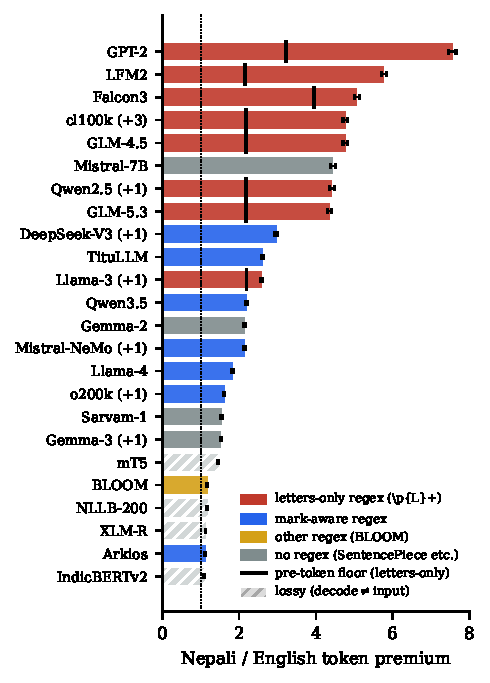
\includegraphics[width=0.95\columnwidth]{fig_audit.pdf}
\caption{Nepali/English token premium of 24 distinct tokenizers (33 released tokenizers; ``+$n$'' counts aliases) on FLORES-200 devtest, with 95\% paired-bootstrap intervals. Black ticks mark the pre-token floor of each letters-only tokenizer: no vocabulary extension can move its bar to the left of the tick.}
\label{fig:audit}
\end{figure}

\paragraph{Every letters-only tokenizer has a floor of at least $2.15\times$.} Eight distinct tokenizers, covering 13 released names including GLM-5.3 and LFM2, use the letters-only class. Their premiums range from $2.58\times$ (Llama-3) to $7.55\times$ (GPT-2), and their pre-token floors from $2.15\times$ to $3.23\times$. Excluding GPT-2, a 2019 model that we include as a historical reference, the premiums of current letters-only models range from $2.58\times$ to $5.77\times$ (LFM2). The seven lossless tokenizers with a mark-aware regex range from $1.12\times$ (Arkios;~\citealp{regmi2026arkios}) to $2.97\times$ (DeepSeek-V3).

\paragraph{Decomposition.} We write each premium as a product of three factors (Appendix~\ref{app:decomp}): a base term, which lies between $0.77$ and $0.80$ for every tokenizer; a \emph{regex factor}, the ratio of Nepali pre-tokens under the tokenizer's own regex to those under the repaired regex; and a \emph{vocabulary factor}, tokens per pre-token, which is the only factor vocabulary extension can lower, and only down to 1. The regex factor is $2.77$--$2.79$ for the Llama-3/Qwen/\texttt{cl100k} pattern, $4.06$ for the GPT-2 and Falcon3 patterns, and $0.98$--$1.02$ for mark-aware tokenizers. For Llama-3 the vocabulary factor is $1.18$, the lowest in the audit, so almost all of its remaining premium is the regex factor. Among mark-aware tokenizers it ranges from $1.43$ (Arkios) to $3.79$ (DeepSeek-V3): fixing the regex is necessary but not sufficient.

\paragraph{Within-family changes.} From Qwen3 to Qwen3.5 the Nepali premium halves ($4.42\times$ to $2.20\times$), with a word branch close to our repaired class~\citep{land2026smallbugs}; from Llama-3 to Llama-4, which adopts \texttt{o200k}'s pattern, it falls from $2.58\times$ to $1.83\times$. The vocabulary also grew in both cases, so these corroborate, but do not replace, the controlled comparison of \S\ref{sec:compression}.

\paragraph{Broken syllables.} Many Nepali tokens begin with a combining mark, which no well-formed Devanagari syllable does: 55\% of Llama-3's, and still 26\% of \texttt{o200k}'s, because BPE also splits within words (Appendix~\ref{app:audit}). \S\ref{sec:compression} shows how the rate moves under each retrofit.
